\documentclass[11pt, oneside]{article}
\usepackage[ngerman]{babel}
\usepackage[ngerman]{datetime}
\usepackage[utf8]{inputenc}

\usepackage[footnotesep=2\baselineskip]{geometry}
\geometry{letterpaper}

\usepackage{subfig}

\usepackage{graphicx}
\graphicspath{ {assets/} }
\usepackage{amssymb}
\usepackage{amsmath}

\usepackage[table,xcdraw]{xcolor}

\usepackage{tikz}
\usetikzlibrary{shapes,arrows}

\usepackage[hyphens]{url} % Break long urls at hyphens
\usepackage{hyperref}

\usepackage{caption}

\usepackage[hang]{footmisc} % Indent multiline footnotes

\usepackage[sc]{mathpazo} % Use the Palatino font
\linespread{1.05} % Line spacing - Palatino needs more space between lines
\usepackage{microtype} % Slightly tweak font spacing for aesthetics

\usepackage[lighttt]{lmodern} % Tweak monospace font
% http://tex.stackexchange.com/a/234020
\ttfamily
\DeclareFontShape{OT1}{lmtt}{m}{it}
     {<->sub*lmtt/m/sl}{}


% Allows abstract customization
\usepackage{abstract}
% Set the "Abstract" text to bold
\renewcommand{\abstractnamefont}{\normalfont\bfseries}
% Set the abstract itself to small italic text
\renewcommand{\abstracttextfont}{\normalfont\small\itshape}

% new line after \paragraph{}
\newcommand{\myparagraph}[1]{\paragraph{#1}\mbox{}\\}

%----------------------------------------------------------------------
%	CODE FORMATTING
%----------------------------------------------------------------------
%
% Usage:
%
%	\begin{lstlisting}[style=custom-xml]
%		...
%	\end{lstlisting}
%
%
%	\lstinputlisting[style=custom-java, caption={AsyncTask Example}]{AsyncTaskExample1.java}
%
\usepackage{listings}
\usepackage{xcolor}
\definecolor{dkgreen}{rgb}{0,0.6,0}
\definecolor{dkred}{rgb}{0.6,0,0}
\definecolor{gray}{rgb}{0.5,0.5,0.5}
\definecolor{mauve}{rgb}{0.58,0,0.82}
\definecolor{gray}{rgb}{0.4,0.4,0.4}
\definecolor{darkblue}{rgb}{0.0,0.0,0.6}
\definecolor{cyan}{rgb}{0.0,0.6,0.6}
\lstset{
	frame=tb,
	aboveskip=3mm,
	belowskip=3mm,
	showstringspaces=false,
	numberblanklines=false,
	columns=flexible,
	basicstyle={\small\ttfamily},
	numberstyle=\tiny\color{gray},
	numbers=left,
	breaklines=true,
	breakatwhitespace=true,
	%title=\lstname, % show the filename of files included with \lstinputlisting;
}
\lstdefinestyle{custom-java}{
	language=Java,
	keywordstyle=\color{blue},
	commentstyle=\color{dkgreen},
	stringstyle=\color{mauve},
	postbreak=\raisebox{0ex}[0ex][0ex]{\ensuremath{\color{gray}\hookrightarrow\space}}
}
\lstdefinestyle{custom-xml}{
	language=XML,
	morestring=[s][\color{mauve}]{"}{"},
	morestring=[s][\color{black}]{>}{<},
	morecomment=[s]{<?}{?>},
	morecomment=[s][\color{dkgreen}]{<!--}{-->},
	stringstyle=\color{black},
	identifierstyle=\color{darkblue},
	keywordstyle=\color{cyan},
	morekeywords={note, to, from, heading, body},
	tabsize=3
}

\renewcommand{\lstlistingname}{Code} %Change "Listing" to "Code" in caption

%----------------------------------------------------------------------
%	INLINECODE
%
%	Usage: \inlinecode{<Code>}
%----------------------------------------------------------------------
%\newcommand{\inlinecode}[1]{\colorbox{gray!10}{\texttt{#1}}}
%\newcommand{\inlinecode}[1]{\textcolor{dkgreen}{\texttt{#1}}}
\newcommand{\inlinecode}[1]{\textcolor{mauve}{\texttt{#1}}}

\renewcommand{\texttt}[1]{%
  \begingroup
  \ttfamily
  \begingroup\lccode`~=`/\lowercase{\endgroup\def~}{/\discretionary{}{}{}}%
  \begingroup\lccode`~=`[\lowercase{\endgroup\def~}{[\discretionary{}{}{}}%
  \begingroup\lccode`~=`.\lowercase{\endgroup\def~}{.\discretionary{}{}{}}%
  \catcode`/=\active\catcode`[=\active\catcode`.=\active
  \scantokens{#1\noexpand}%
  \endgroup
}

%----------------------------------------------------------------------
%	BOXES
%----------------------------------------------------------------------
%
% Usage:
%	\begin{mdframed}[style=highlightbox]
%		...
%	\end{mdframed}
%
\usepackage[framemethod=tikz]{mdframed} %background
\mdfdefinestyle{highlightbox}{%
	backgroundcolor=gray!20,
	linewidth=0pt,
	innertopmargin=10pt,
	innerbottommargin=10pt,
	frametitleaboveskip=5pt,
	roundcorner=5pt
}

\mdfdefinestyle{advicebox}{%
	linecolor=gray!20,
	linewidth=1pt,
	innertopmargin=10pt,
	innerbottommargin=10pt,
	frametitleaboveskip=5pt,
	roundcorner=5pt
}

\mdfdefinestyle{example}{settings={\@mkboth{\mdf@frametitle}{\mdf@frametitle}}}










%----------------------------------------------------------------------
%	TITLE SECTION
%----------------------------------------------------------------------

\begin{document}
\hypersetup{pageanchor=false}
\thispagestyle{empty}

\begin{figure}
\centering

\includegraphics[height=80pt]{hska_logo.png}
\end{figure}

\begin{center}

\large{Fakultät für Informatik- und Wirtschaftsinformatik \\
der Hochschule Karlsruhe - Technik und Wirtschaft \\}
\vspace{5mm}
\large{\textsc{IW912 App-Programming WS2016/17}} \\
\vspace{3mm}
\fontsize{16pt}{7pt}\selectfont\textbf{Aufgaben Klausurbonus} \\
\vspace{5mm}
Jan Sauerwein\\
\vspace{10mm}
\large{\textbf{Ausarbeitung}} \\
\vspace{10mm}
\textsc{Jonas Rottmann}\\
Matrikel Nr.: 44501\\
\href{mailto:rojo1020@hs-karlsruhe.de}{rojo1020@hs-karlsruhe.de}\\[2mm]

\end{center}
\newpage

%----------------------------------------------------------------------
%	TOC
%----------------------------------------------------------------------

\microtypesetup{protrusion=false} % disables protrusion locally in the document
\tableofcontents % prints Table of Contents
\microtypesetup{protrusion=true} % enables protrusion
\newpage

%----------------------------------------------------------------------
%	MAIN CONTENTS
%----------------------------------------------------------------------
\pagenumbering{arabic}

\section{Layout Konzept}
\subsection{Layout}
\begin{figure}[h]
	\begin{center}
	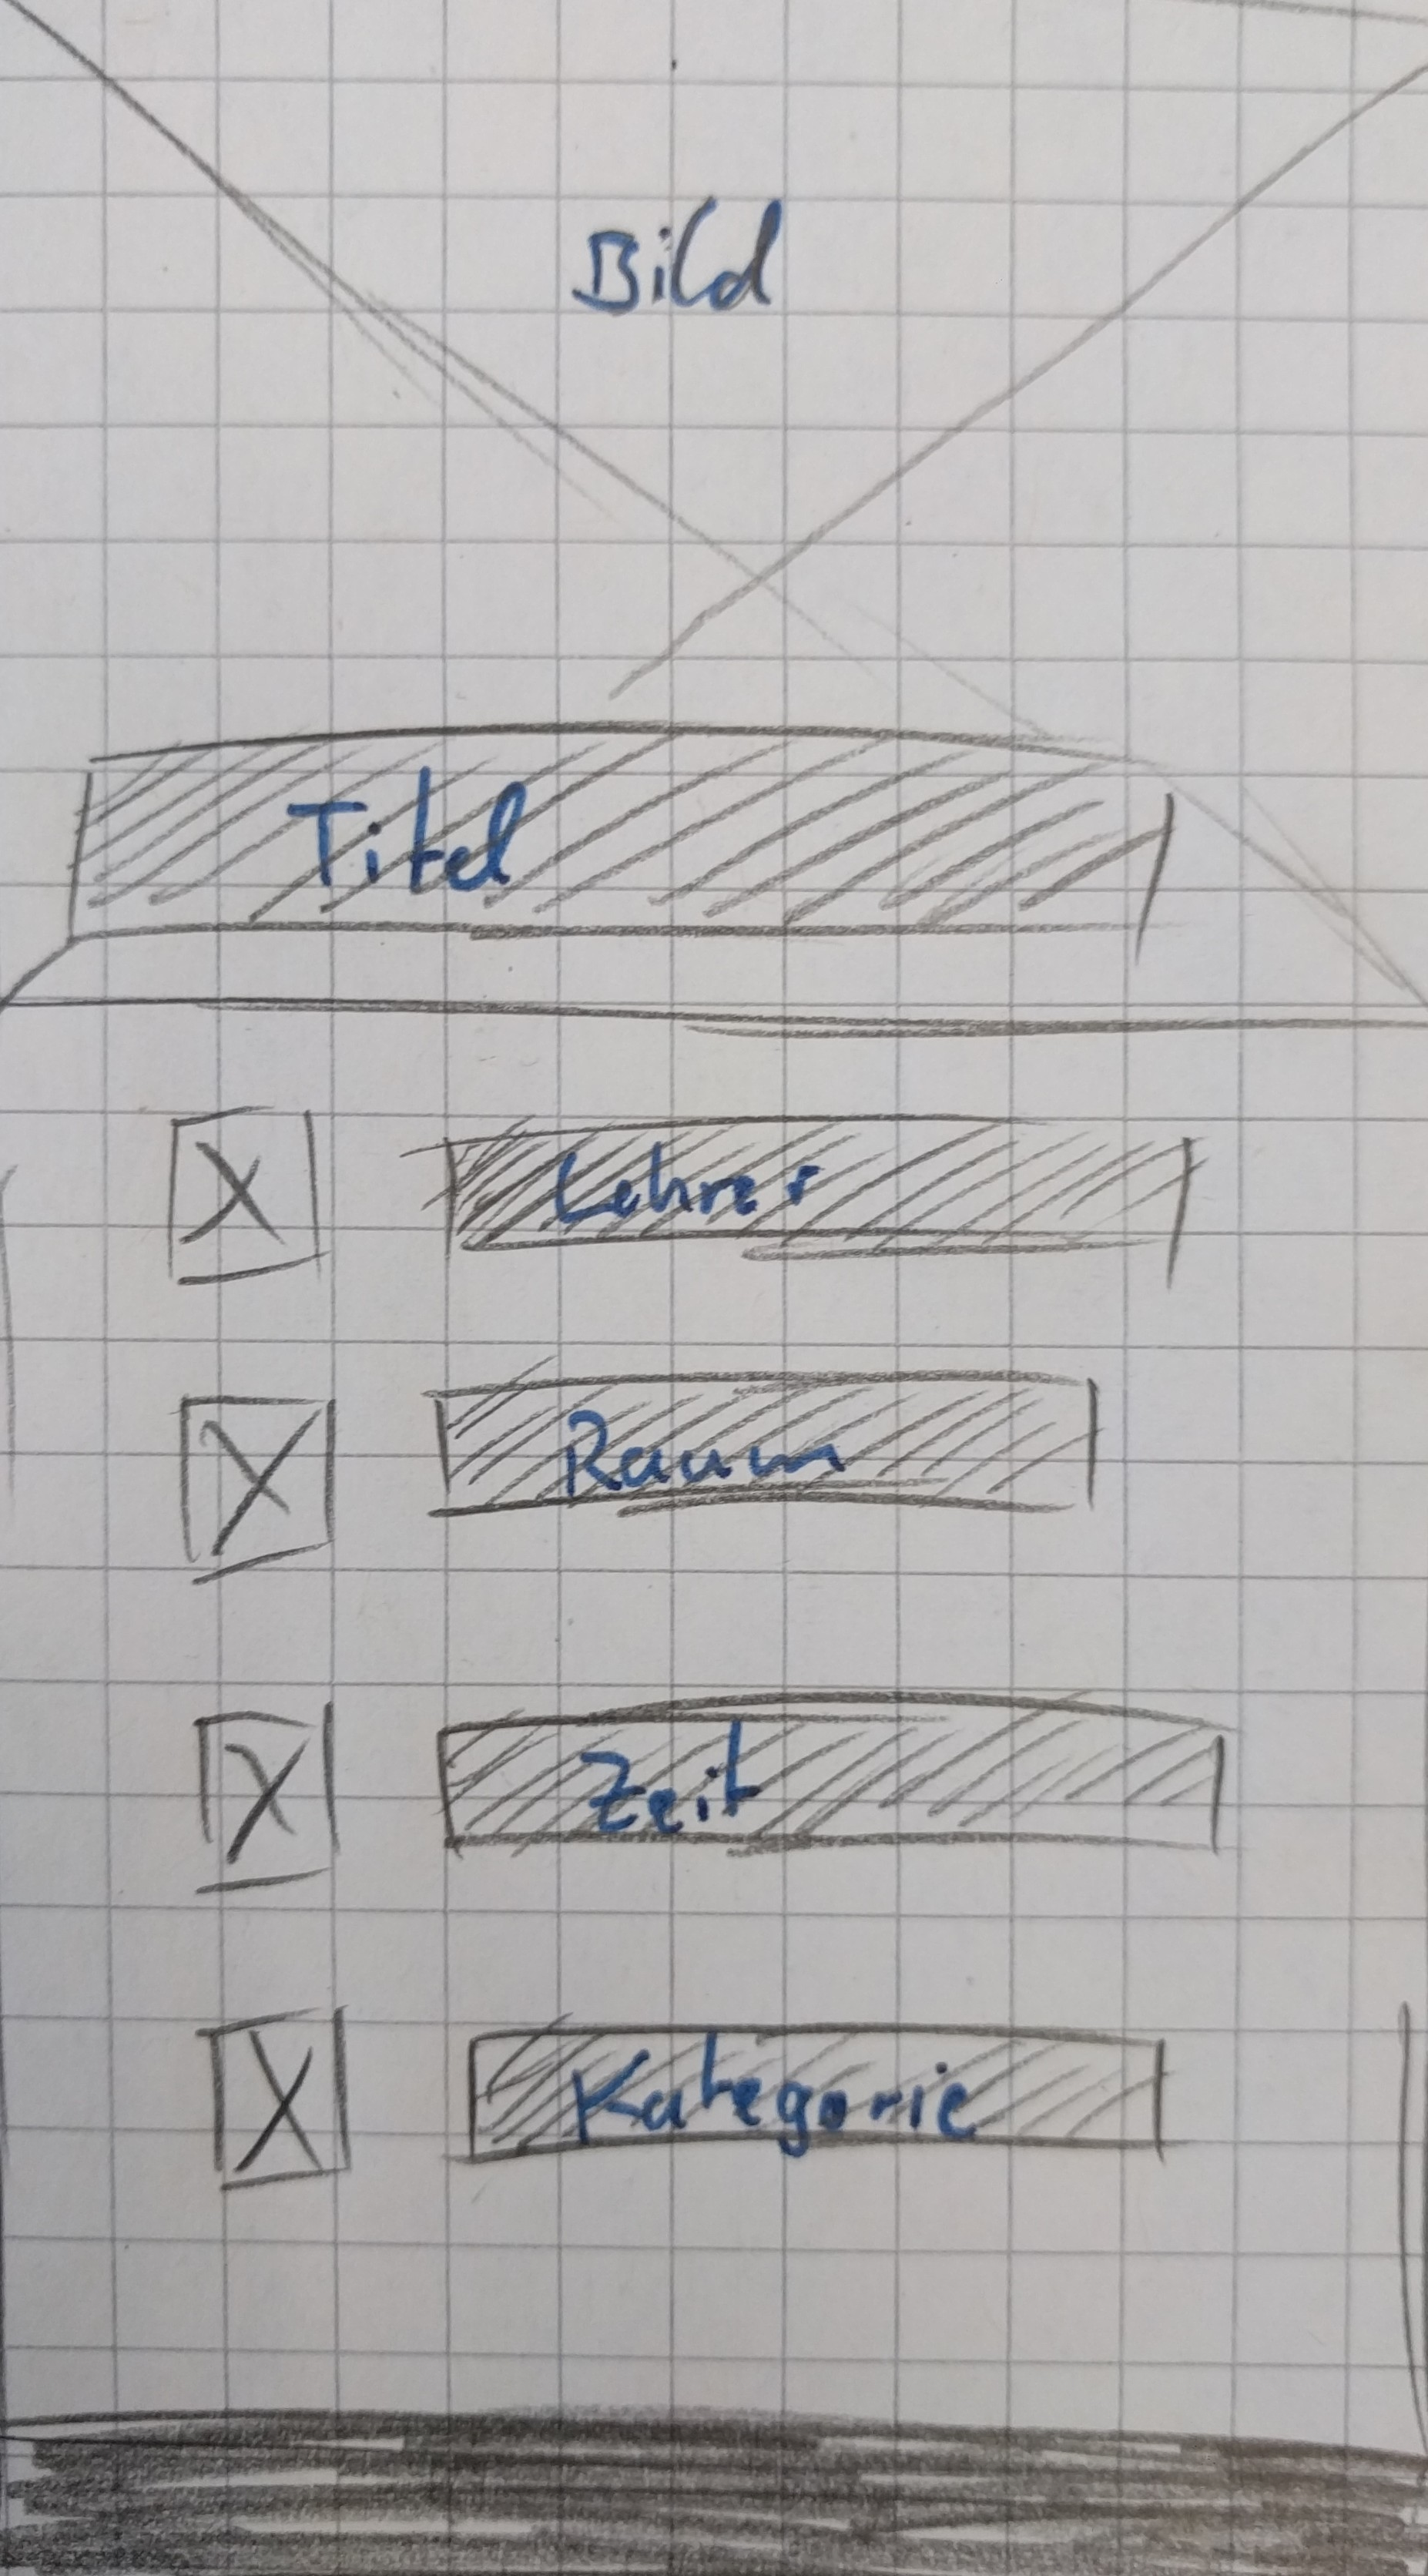
\includegraphics[scale=0.1]{sketch_1}
	\end{center}
	\caption{Layout Entwurf - Portrait}
	\label{fig:sketch1}
\end{figure}


\subsection{Größen und Orientierung}
Die Landscape-Ansicht für Phones ist in Abbildung \ref{fig:sketch2} zu sehen.
\begin{figure}[h]
	\begin{center}
	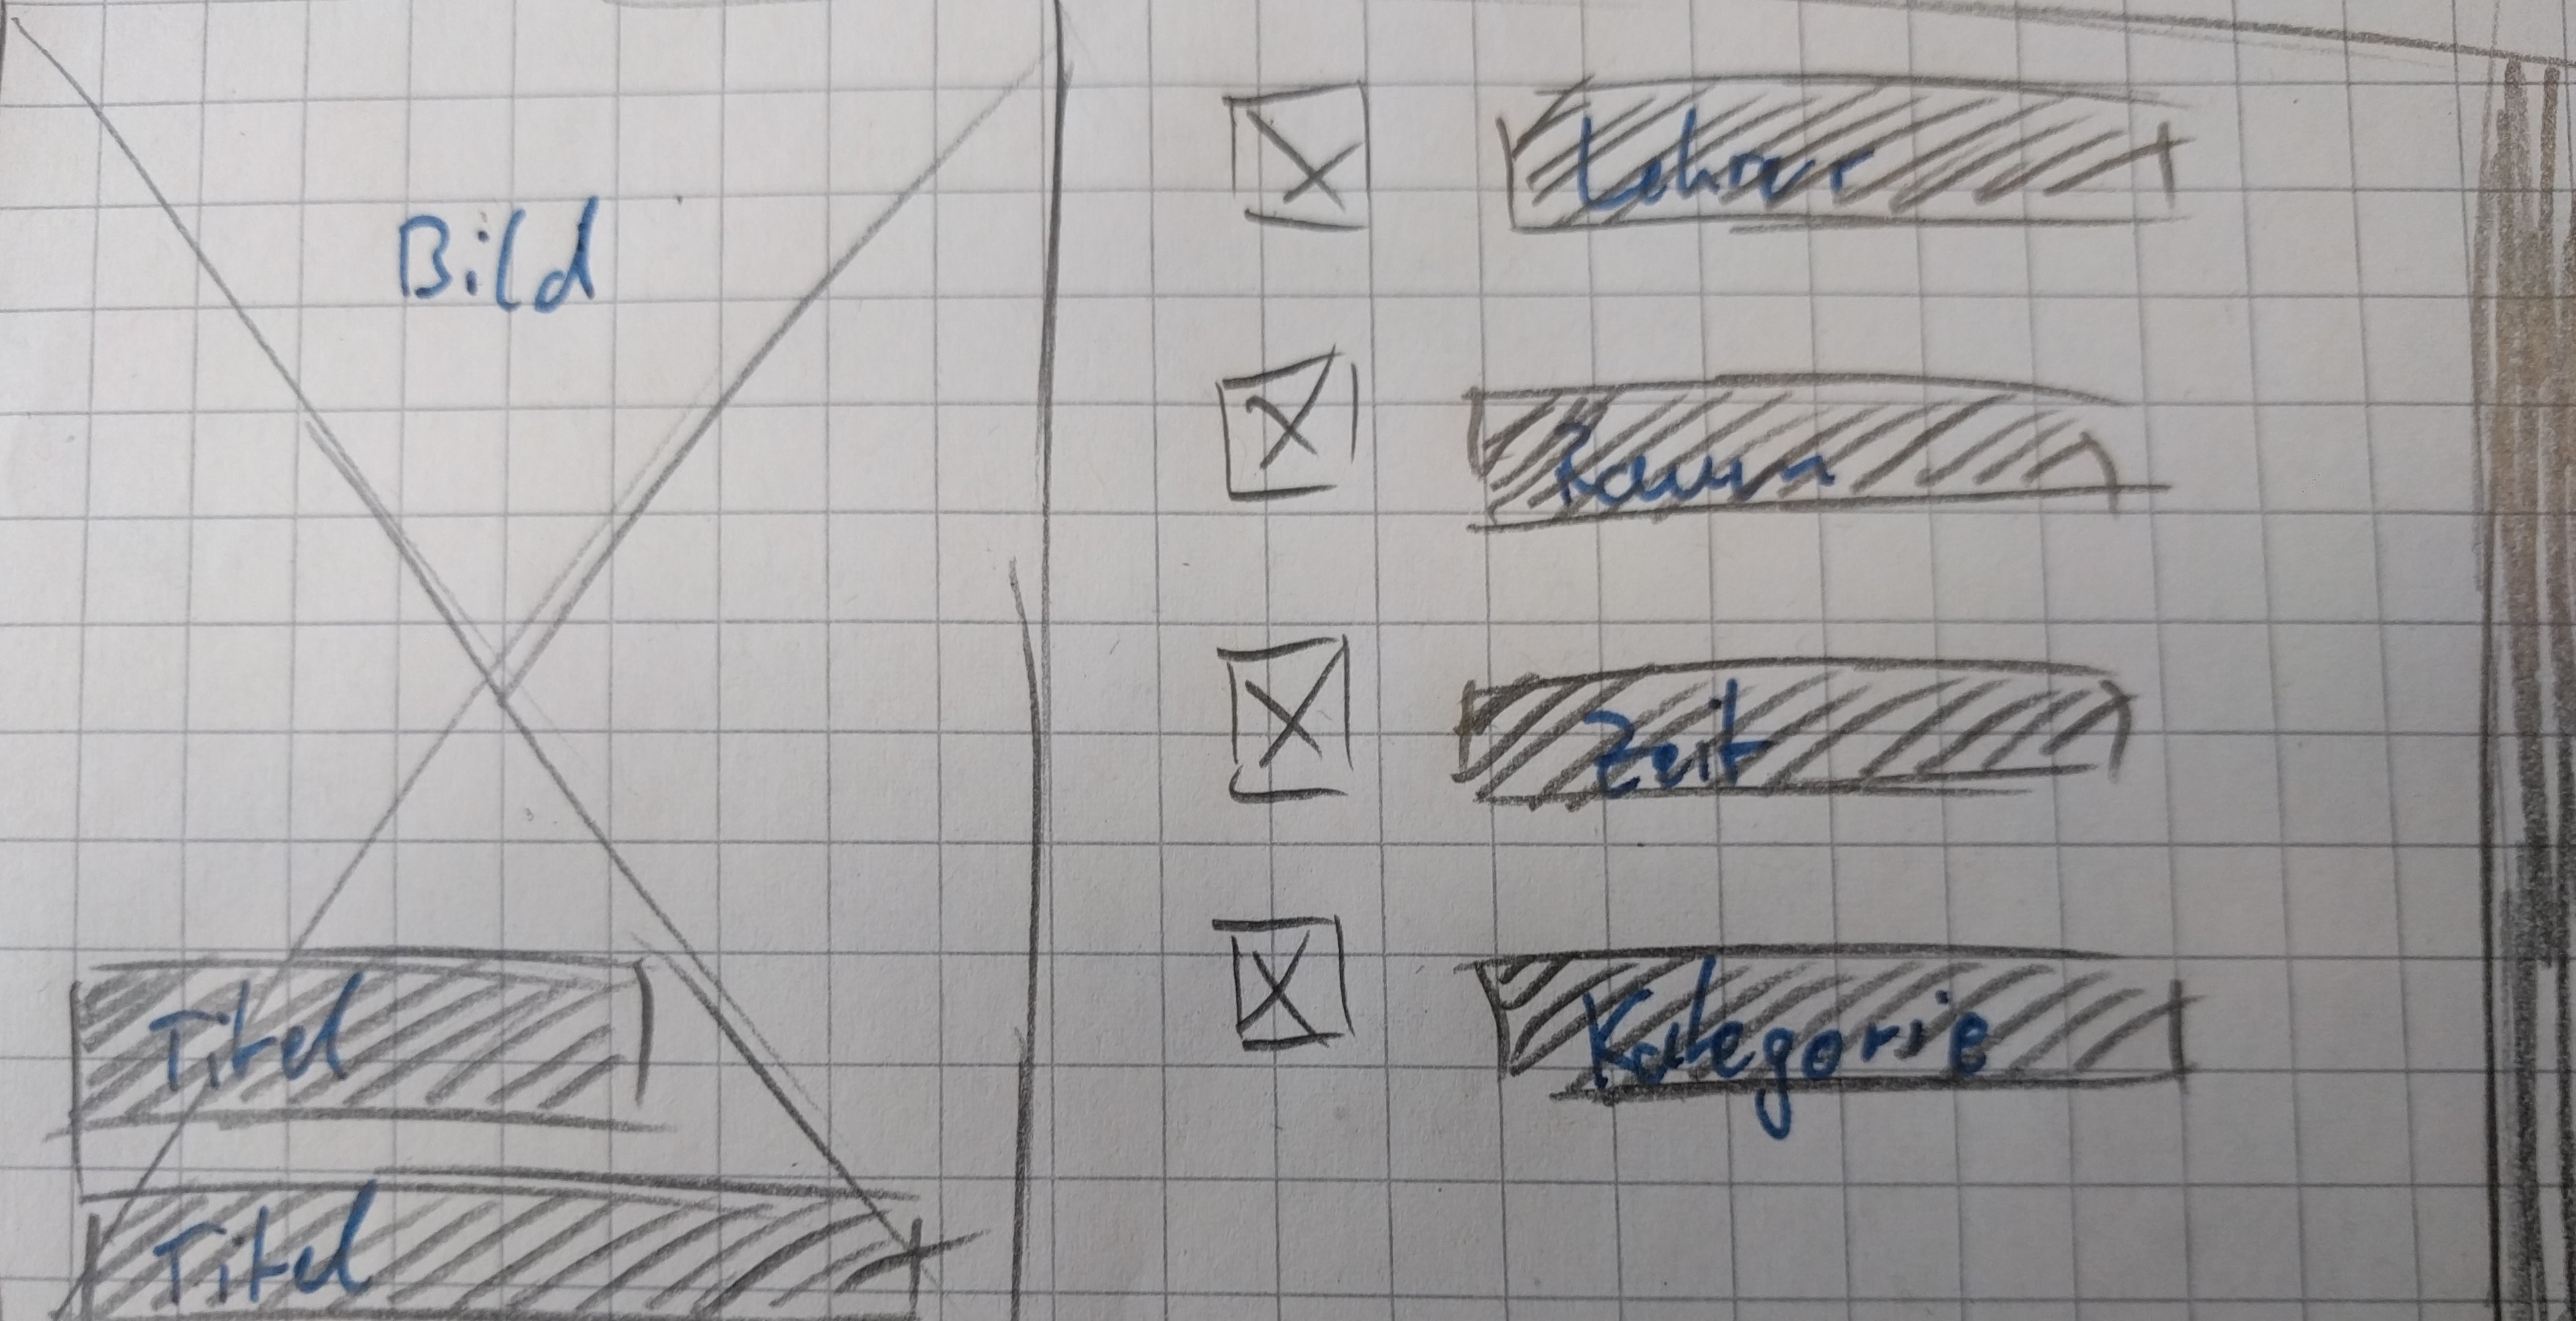
\includegraphics[scale=0.1]{sketch_2}
	\end{center}
	\caption{Layout Entwurf - Landscape}
	\label{fig:sketch2}
\end{figure}
Bei der Tablet-Ansicht (Abbildung \ref{fig:sketch_tablet}) wird das Layout aus Abbildung \ref{fig:sketch1} wiederverwendet.
\begin{figure}[h]
	\begin{center}
	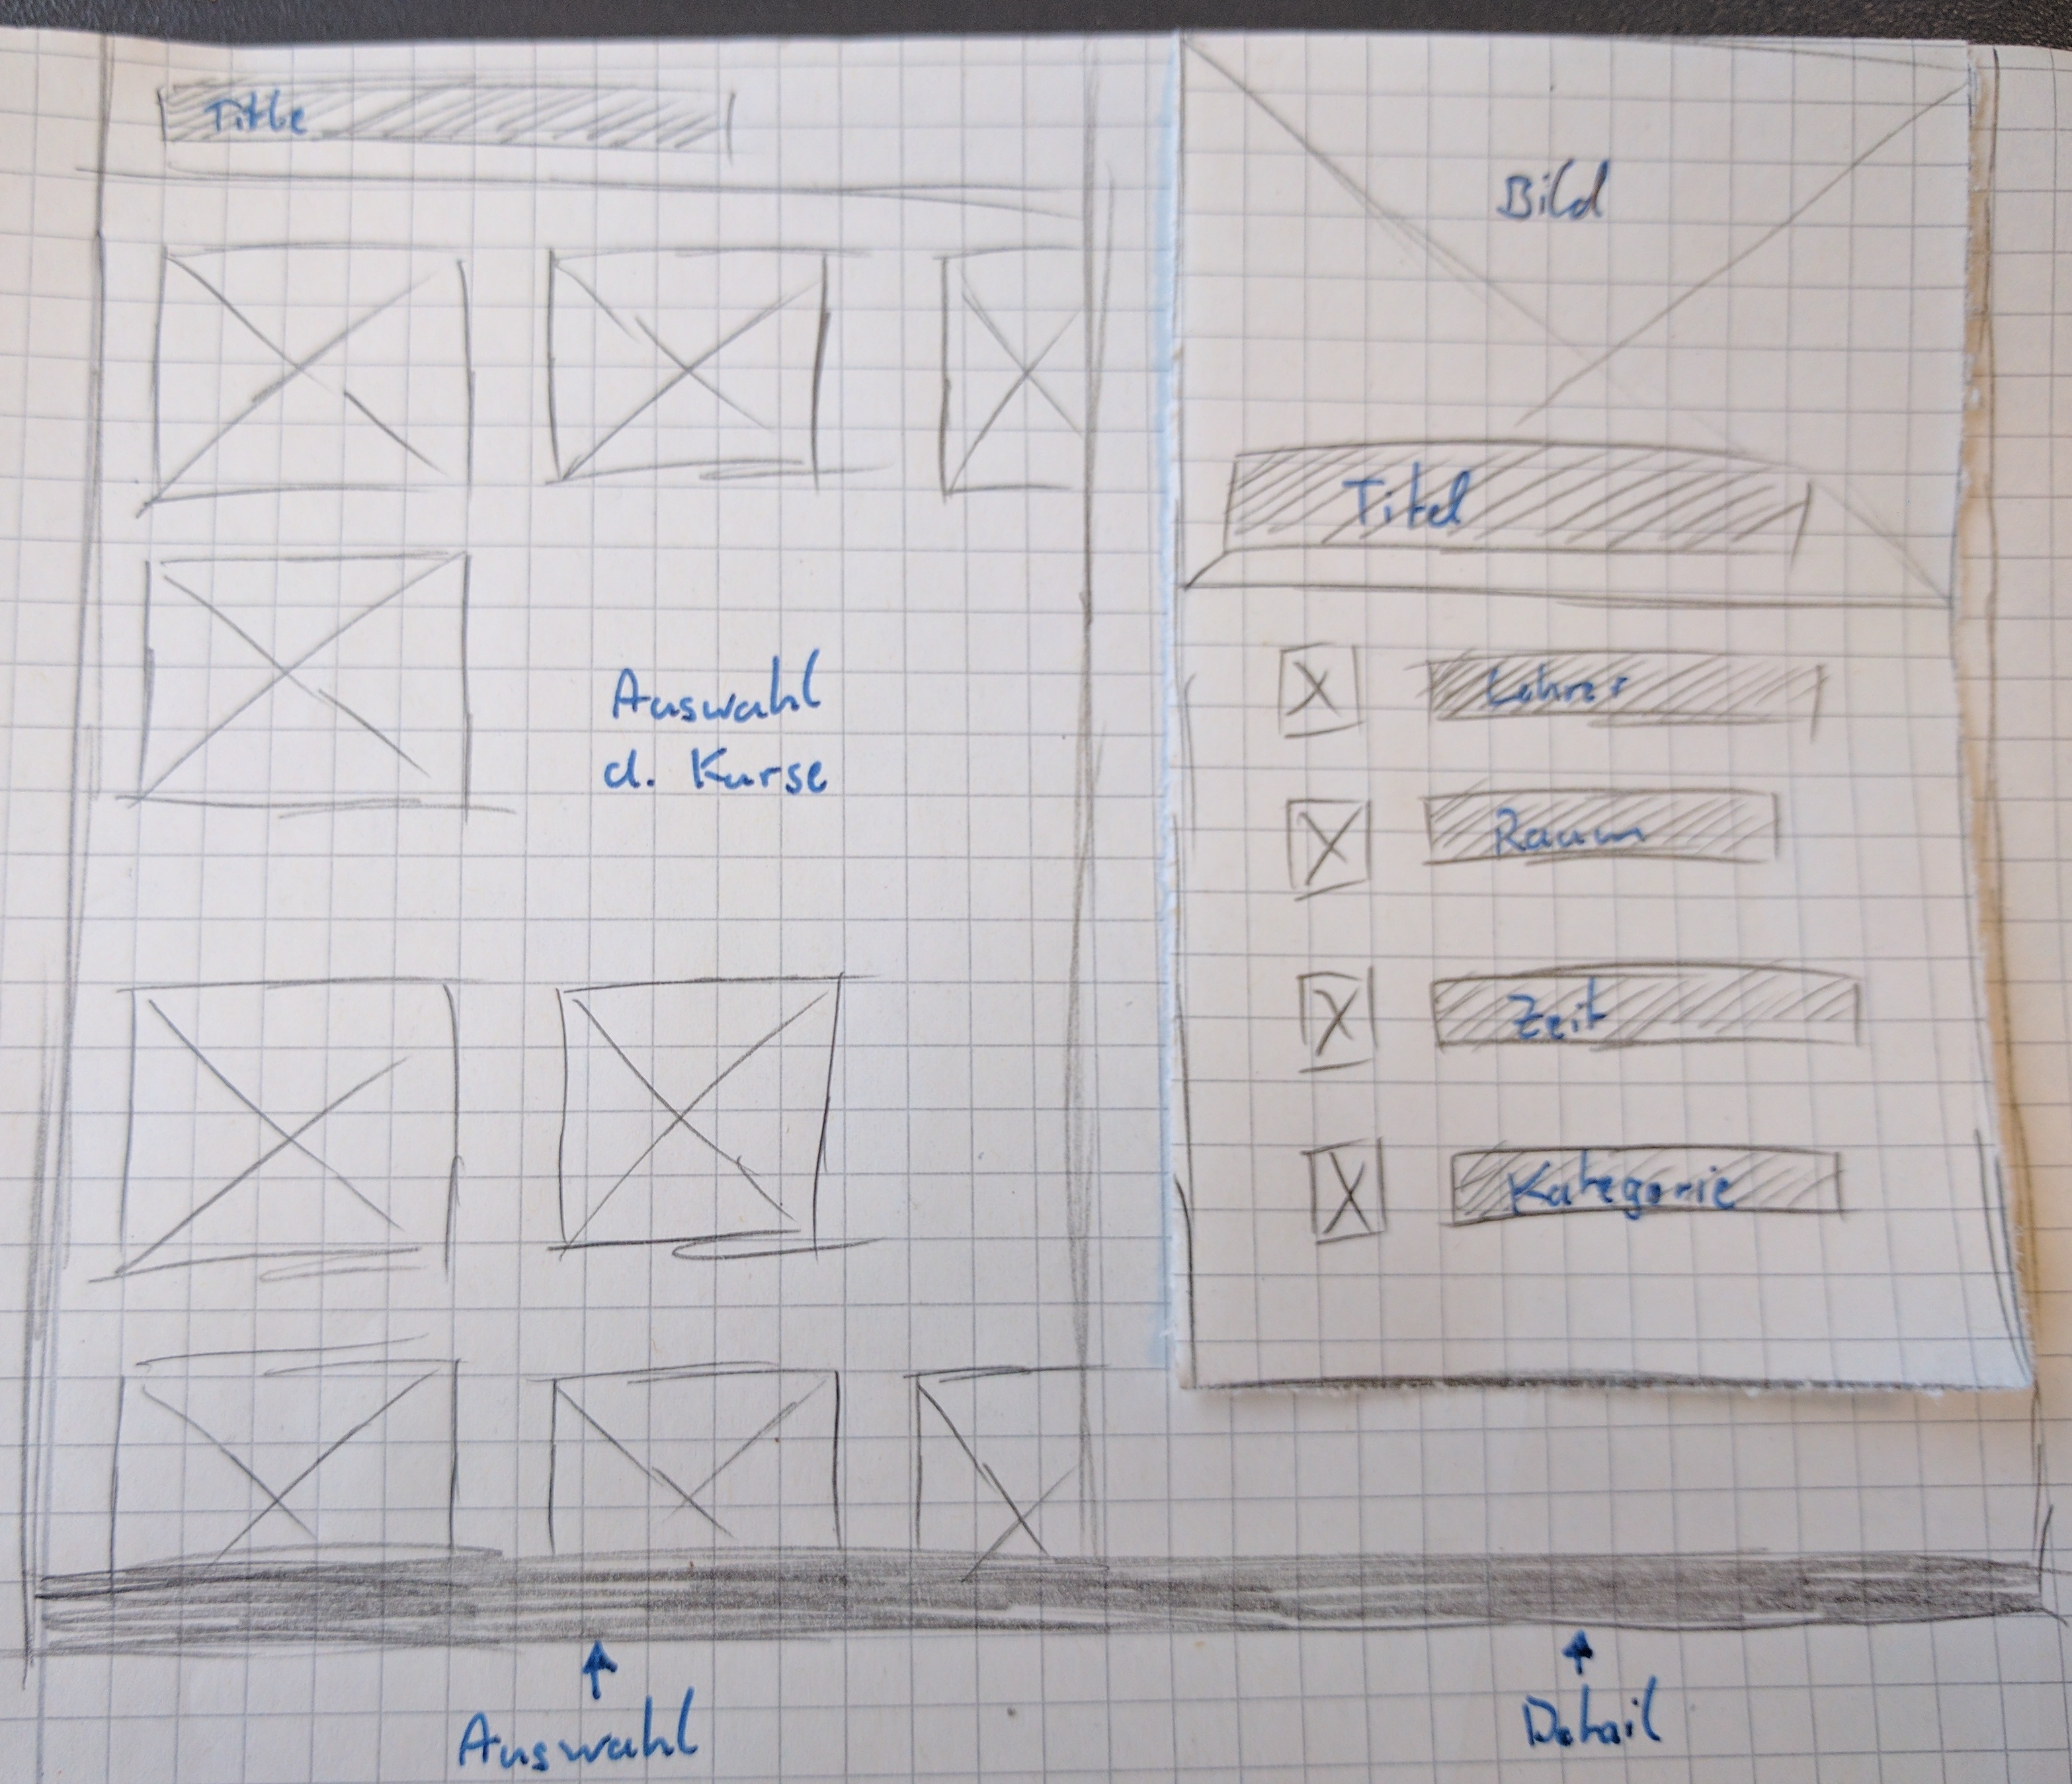
\includegraphics[scale=0.09]{sketch_tablet}
	\end{center}
	\caption{Layout Entwurf - Tablet}
	\label{fig:sketch_tablet}
\end{figure}


\subsection{Begründung}
Die Detailansicht bietet mit dem großen Bild eine gute Übersichtlichkeit, außerdem wird das gesamte Layout in der Farbe, der Kategorie, des ausgewählten Angebots eingefärbt (siehe Abbildungen \ref{fig:fab} und \ref{fig:alert}), was eine zusäzuliche Orientierungshilfe für die Grundschulkinder bietet. Im der Landscape-Orientierung werden Bild und Infos zum Angebot nebeneinander angezeigt um auch hier durch ein großes Bild möglichst viel Übersichtlicheit zu bieten ohne unnötig scrollen zu müssen.

Für Tablets wird das gleiche Layout benutzt (später Neu-Anordnung von Fragments), da ich mich für ein Master/Detail-Flow Navigations Pattern\footnote{\url{https://developer.android.com/training/implementing-navigation/descendant.html\#master-detail}, [Online; \formatdate{05}{02}{2017}]} entschieden habe. Bei Tablets wird nicht zwischen Portrait und Landscape unterschieden, da in beiden Orientierungen genug Platz zur Verfügung steht.



\section{Layout Umsetzung}
\subsection{Layout}
Die Layouts sind als \inlinecode{fragment\_detail.xml} in den entsprechenden Ordnern zu finden.

\subsection{Inhalte}
Zu zuweisung der Werte erfolgt in der Klasse \inlinecode{DetailFragment.java} und zwar in der Callback-Methode \inlinecode{onCreateView()}.
\begin{lstlisting}[language=Java, firstnumber=132]
fab.setActivated(course.getStarred());
backdrop.setImageDrawable(ContextCompat.getDrawable(getActivity(), Icon.getIconResId(course.getIcon())));
if (course.getTeacher() != null) {
    teacherText.setText(course.getTeacher());
} else {
    teacherRow.setVisibility(GONE);
}
if (course.getRoom() != null) {
    roomText.setText(course.getRoom());
} else {
    roomRow.setVisibility(GONE);
}
timeText.setText(TimeSlot.getTimeSlotForId(course.getTimeslot()));
catText.setText(Category.getCategoryStringForId(course.getCategory()));
\end{lstlisting}
Die entsprechenden Werte weden aus \inlinecode{course} - einer Instanz der Klasse \inlinecode{de.jonasrottmann.planerapp.data.model.Couse} - abgeholt, die dem \inlinecode{DetailFragment.java} als \inlinecode{Parcelable} in den Arguments übergeben wird.


\section{Layout und Adapter}
\subsection{Layout}
Die entsprechenden Layouts sind in \inlinecode{fragment\_overview.xml}, \inlinecode{item\_courses\_row.xml} (eine Zeile des äußeren \inlinecode{RecyclerView}, die einen zweiten \inlinecode{RecyclerView} enthält) sowie \inlinecode{item\_course.xml} (die rechteckige Vorschaukarte eines speziellen Kurs) zu finden.
Bidirektionales Scrollen wurde also durch verschachtelte \inlinecode{RecyclerView}s umgesetzt.
Die Mittagspause um 12:00 Uhr, in der keine Kurse angeboten werden wurde durch einen zweiten ViewHolder des äußeren \inlinecode{RecyclerView} umgesetzt. Dies ist in der Klasse \inlinecode{OverviewAdapter.java} zu sehen.
\begin{lstlisting}[language=Java, firstnumber=42]
@Override
public int getItemViewType(int position) {
    return position == 4 ? VIEWTYPE_TEXT : VIEWTYPE_COURSES;
}
\end{lstlisting}
Die Methode \inlinecode{getItemViewType()} gibt den entsprechenden Typ des anzuzeigenden ViewHolders zurück. In \inlinecode{onCreateViewHolder()} und \inlinecode{onBindViewHolder()} wird dann der passende Typ erzeugt bzw. befüllt.

\subsection{Adapter}
Dieser Schritt wurde durch das Befüllen mit Hilfe eines \inlinecode{Cursor} ersetzt. Die Adapter sind als \inlinecode{OverviewAdapter.java} sowie \inlinecode{OverviewRowAdapter.java} im Projekt zu finden.


\section{Interaktion}
\subsection{Layouts verbinden}
Das Anklicken eines Angebots wird im \inlinecode{OverviewAdapter}, also dem 
Adapter des äußeren \inlinecode{RecyclerView}, umgesetzt, indem in \inlinecode{onBindViewHolder()} der Adapter des inneren \inlinecode{RecyclerView} (\inlinecode{OverviewRowAdapter}) initialisiert und ein \inlinecode{View.OnClickListener} übergeben wird.
\begin{lstlisting}[language=Java, firstnumber=78]
OverviewRowAdapter adapter = new OverviewRowAdapter(cursor1, context, new View.OnClickListener() {
    @Override
    public void onClick(View v) {
        int pos = ((ViewHolderCoursesRow) holder).recycler.getChildAdapterPosition(v);
        Cursor cursor2 = ((OverviewRowAdapter) ((ViewHolderCoursesRow) holder).recycler.getAdapter()).getCursor();
        cursor2.moveToPosition(pos);
        contract.onCourseClicked(cursor2.getInt(Index.COLUMN_ID));
    }
});
\end{lstlisting}
Dieser leitet die Information an \inlinecode{contract} (die Activity) weiter, welche die entsprechende \inlinecode{FragmentTransaction} ausführt um die Detail-Ansicht anzuzeigen/auszutauschen (je nachdem ob Phone oder Tablet).

\subsection{Dynamische Daten}
Da in \inlinecode{contract.onCourseClicked()} die ID des angeklickten Kurses übergeben wird, kann die Activity dem \inlinecode{DetailFragment} die benötigten Informationen des anzuzeigenden Kurs übergeben.


\section{Adapter und DB}
\subsection{Datenbank}
Die Befehle um die Datanbank (nur für Veranstaltungen am Montag) anzulegen sind in der Datei \inlinecode{seed.sql} im \inlinecode{assets/} Ordner vorhanden. In der \inlinecode{onCreate()}-Methode des \inlinecode{CourseDatabaseHelper} werden diese Befehle nacheinander ausgeführt, und so die Datenbank erstellt.
\begin{lstlisting}[language=Java, firstnumber=38]
@Override
public void onCreate(SQLiteDatabase db) {
    AssetManager am = context.getAssets();
    try {
        InputStream inputStream = am.open("seed.sql");
        ByteArrayOutputStream byteArrayOutputStream = new ByteArrayOutputStream();
        int i;
        i = inputStream.read();
        while (i != -1) {
            byteArrayOutputStream.write(i);
            i = inputStream.read();
        }
        inputStream.close();

        String[] queries = byteArrayOutputStream.toString().split(";\n");
        for (String query : queries) {
            db.execSQL(query);
        }
    } catch (IOException e) {
        e.printStackTrace();
    }
    am.close();
}
\end{lstlisting}

\subsection{Adapter}
Siehe \inlinecode{OverviewAdapter.java} sowie \inlinecode{OverviewRowAdapter.java}.


\section{Loader und ContentProvider}
\subsection{ContentProvider als Fassade}
Siehe \inlinecode{CourseContentProvider}.

\subsection{Loader}
Im \inlinecode{OverviewFragment} werden die \inlinecode{LoaderManager.LoaderCallbacks<Cursor>} implementiert und in \inlinecode{onCreate()} der \inlinecode{Loader} initialisiert. In \inlinecode{onLoadFinished()} wird dann der \inlinecode{Cursor} des äußeren Adapter ausgetauscht und dadurch \inlinecode{notifyDataSetChanged()} auf dem \inlinecode{RecyclerView} aufgerufen (siehe \inlinecode{CursorRecyclerViewAdapter}).
\begin{lstlisting}[language=Java, firstnumber=70]
@Override
public void onLoadFinished(Loader<Cursor> loader, Cursor data) {
    this.cursor = data;
    ((CursorRecyclerViewAdapter) this.recycler.getAdapter()).changeCursor(this.cursor);
}
\end{lstlisting}


\section{ContentProvider und Datenänderungen}
\subsection{ContentProvider}
Dies wird im \inlinecode{CourseContentProvider} durch die \inlinecode{update()}-Methode realisiert. 
\begin{lstlisting}[language=Java, firstnumber=92]
@Override
public int update(@NonNull Uri uri, ContentValues values, String selection, String[] selectionArgs) {
    if (URI_MATCHER.match(uri) == COURSE_ID) {
        Course course;
        Cursor courseCursor = database.getCourse(Integer.parseInt(uri.getPathSegments().get(1)), DatabaseContract.Course.ALL_COLUMNS, null, null, null);
        if (courseCursor != null && courseCursor.moveToFirst()) {
            course = new Course(courseCursor);
        } else {
            throw new IllegalArgumentException("No course with this id.");
        }
        if (values.getAsInteger(DatabaseContract.Course.Columns.COLUMN_STAR) == 1) {
            // Course should be starred
            // Get stared course for this timeslot
            Cursor starredCourses = database.getAllCourses(DatabaseContract.Course.ALL_COLUMNS,
                DatabaseContract.Course.Columns.COLUMN_WEEKDAY + " = ? AND " + DatabaseContract.Course.Columns.COLUMN_TIMESLOT + " = ? AND " + DatabaseContract.Course.Columns.COLUMN_STAR + " = ?",
                new String[] {
                    String.valueOf(course.getWeekday()), String.valueOf(course.getTimeslot()), String.valueOf(1)
                }, null);
            if (starredCourses == null || starredCourses.getCount() != 0) {
                throw new IllegalStateException("Only one starred course per timeslot allowed.");
            } else {
                // Set star
                getContext().getContentResolver().notifyChange(uri, null);
                return database.updateCourse(course.getId(), values);
            }
        } else {
            // Remove star
            getContext().getContentResolver().notifyChange(uri, null);
            return database.updateCourse(course.getId(), values);
        }
    } else {
        throw new IllegalArgumentException("Not allowed to update multiple courses at once.");
    }
}
\end{lstlisting}
Dass nun die markierten Angebote immer als erstes zurückgegeben werden wird in der \inlinecode{query()}-Methode durch eine Sortierung 
\inlinecode{DatabaseContract.Course.Columns.COLUMN\_STAR + " DESC"} sichergestellt.



\section{Markieren von Angeboten}
\subsection{Interkation}
Die Detailansicht in \inlinecode{fragment\_detail.xml} enthält einen \inlinecode{FloatingActionButton}, über den eine Markierung gesetzt bzw. aufgehoben werden kann.
\begin{figure}[h]
	\begin{center}
	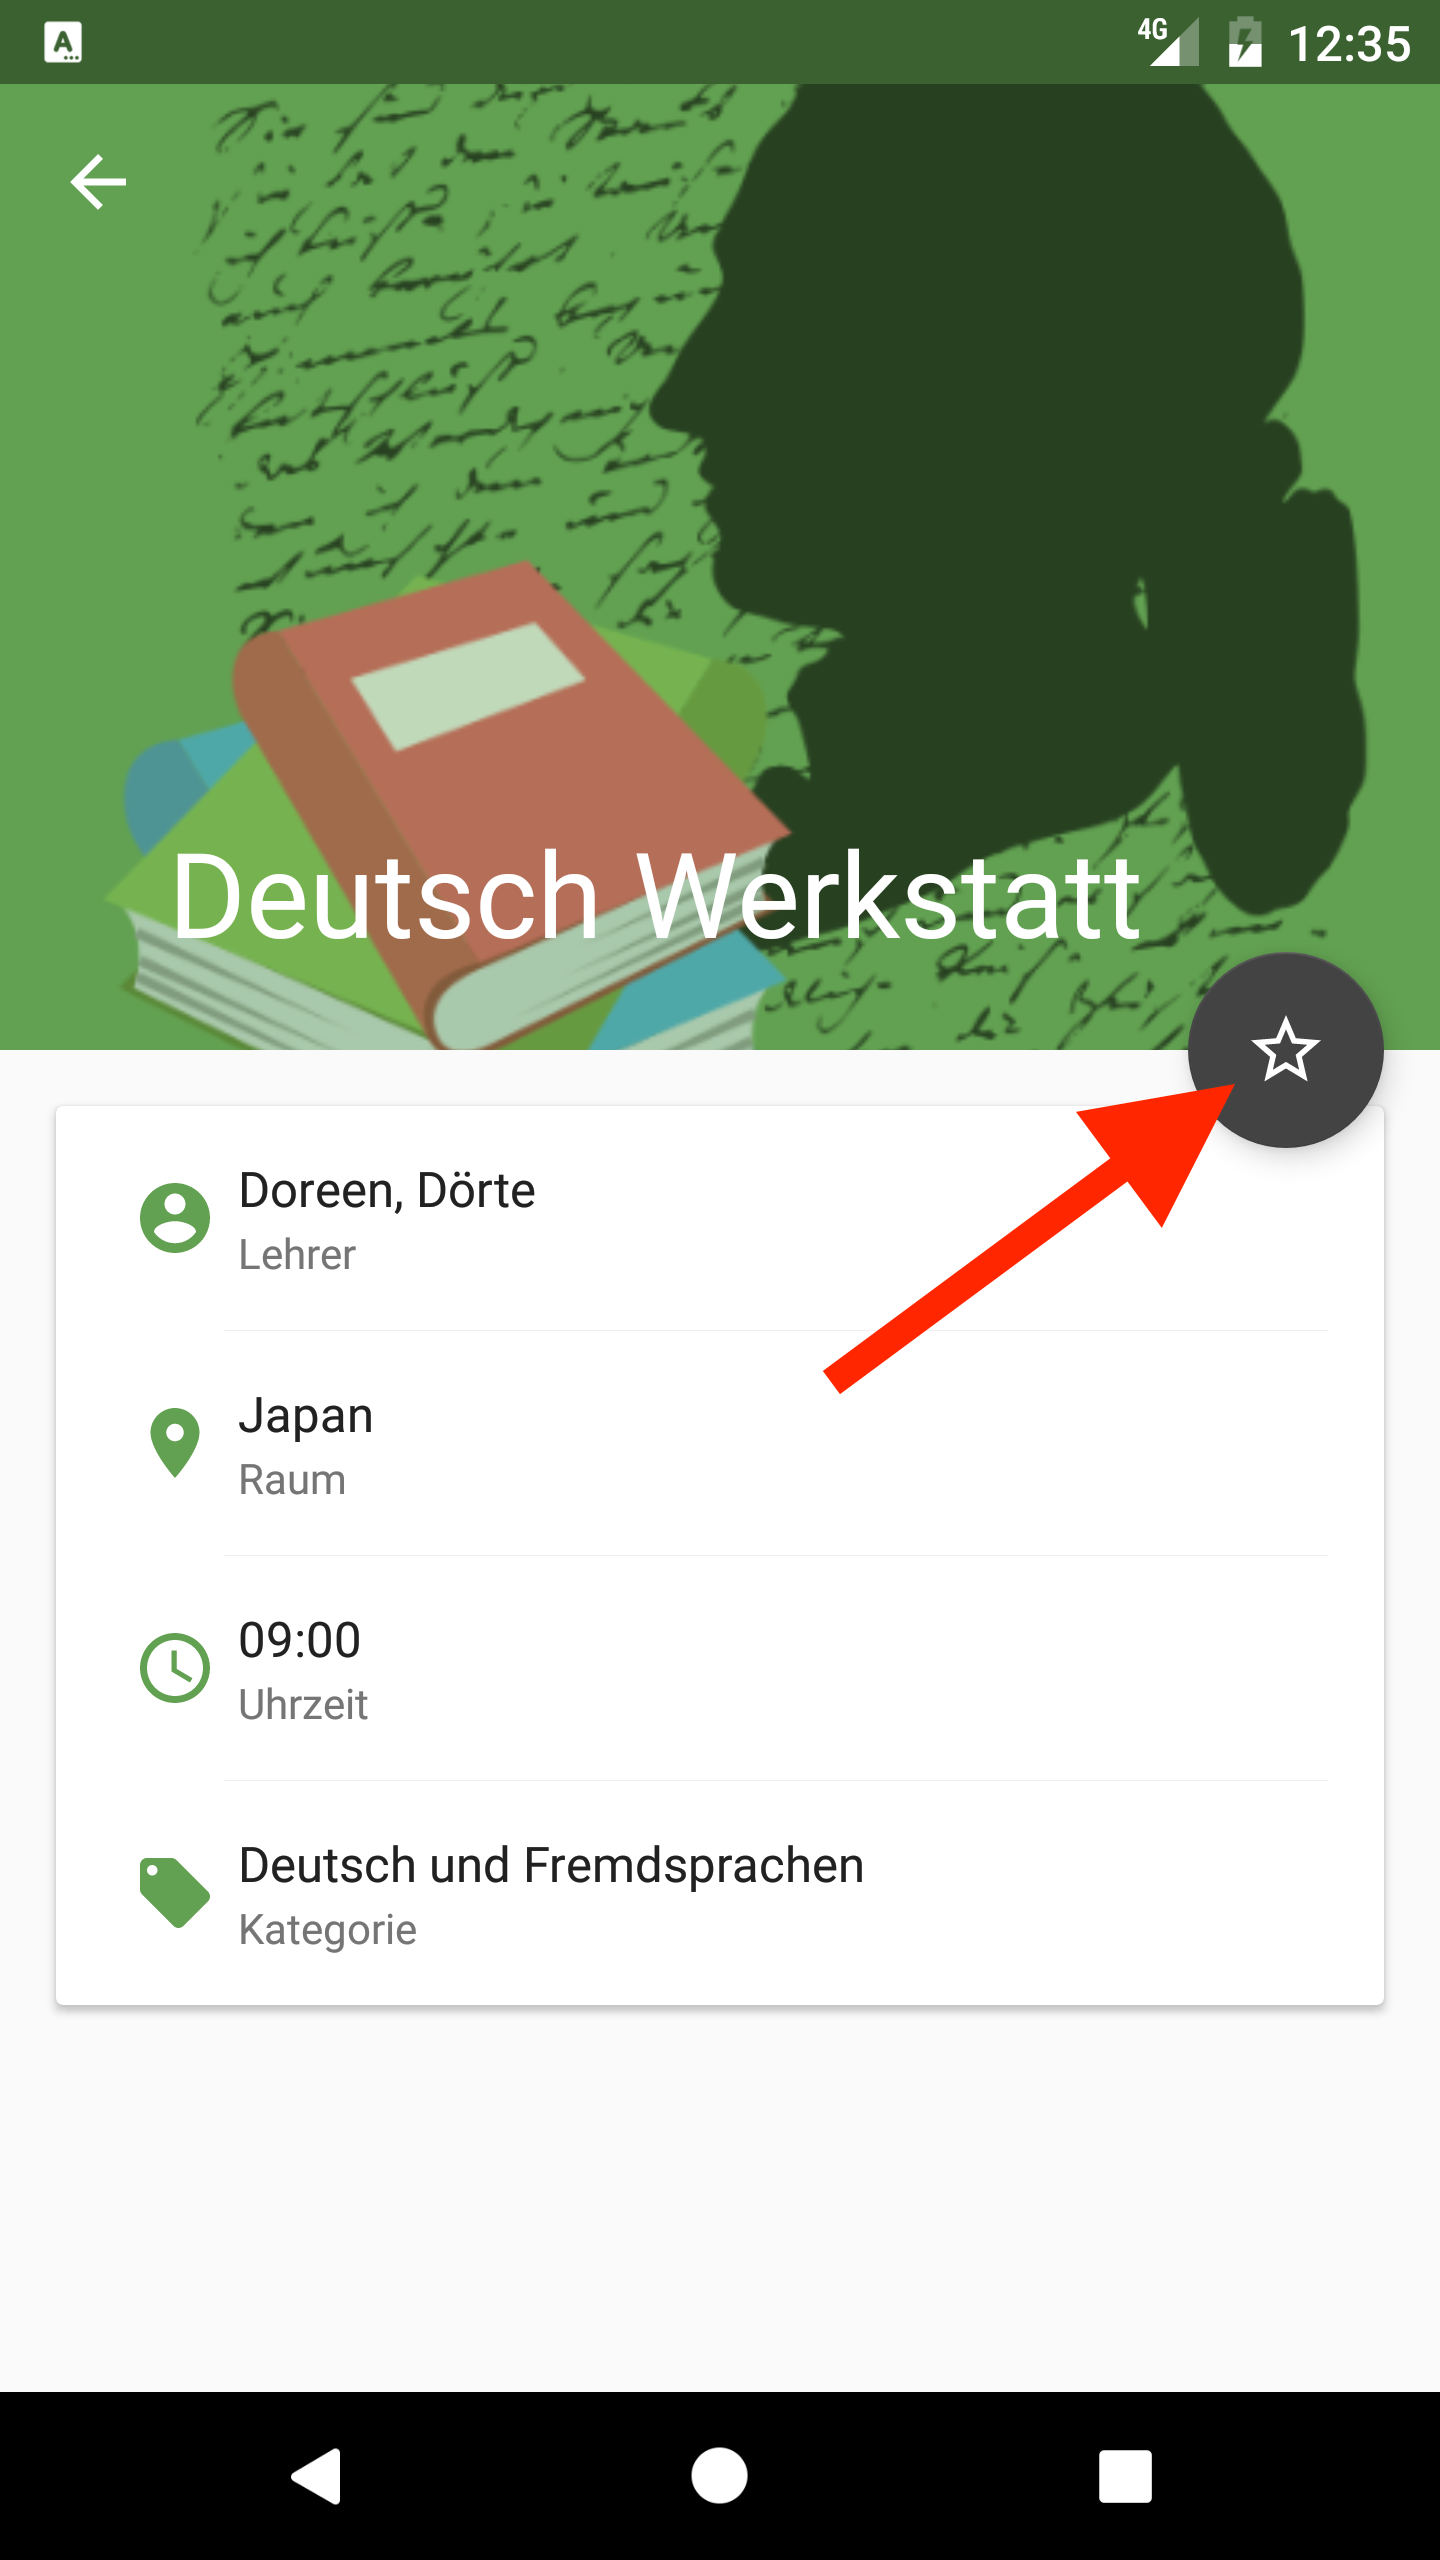
\includegraphics[scale=0.075]{screen_fab}
	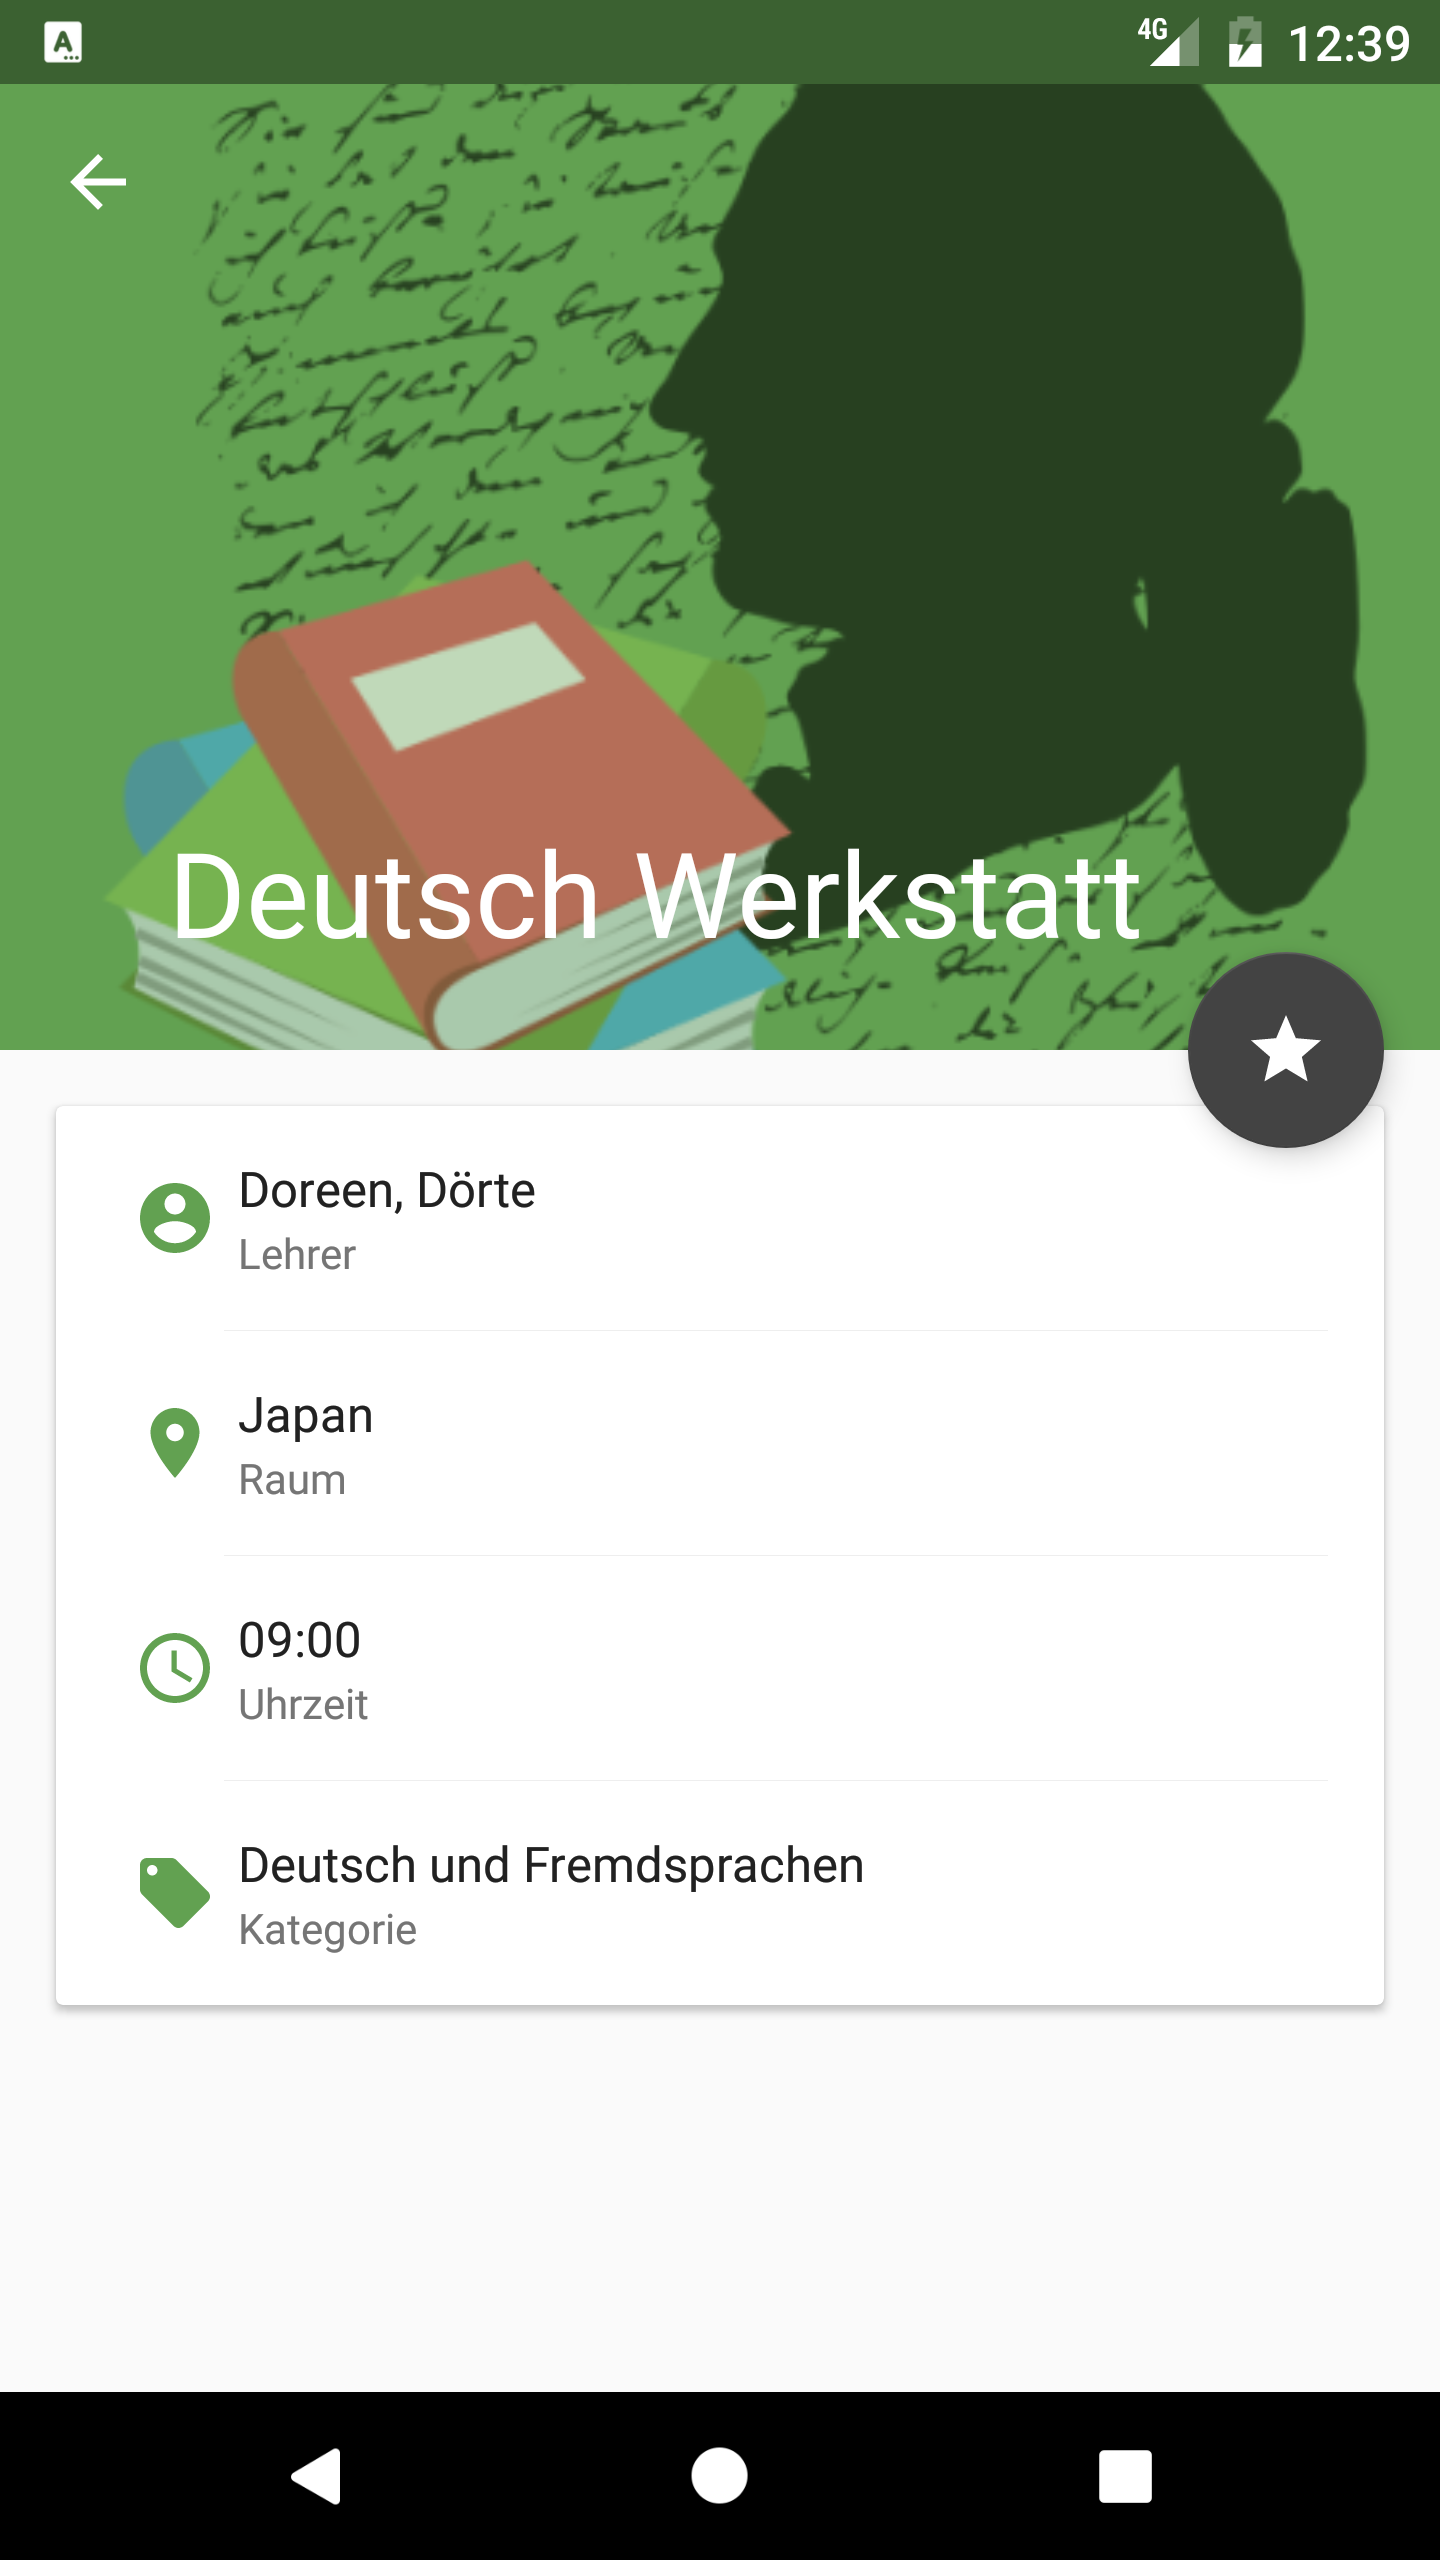
\includegraphics[scale=0.075]{screen_fab_active}
	\end{center}
	\caption{Detailansicht mit Buttom zur Markierung eines Angebots}
    \label{fig:fab}
\end{figure}

\subsection{Aktion}
Durch \inlinecode{toggleStarCourseClicked()} in \inlinecode{DetailFragment} wird geprüft ob schon ein Angebot in diesem Zeitfenster markeirt wurde, wenn ja, wird ein \inlinecode{AlertDialog} (siehe Abbildung \ref{fig:alert}) angezeigt. Durch \inlinecode{toggleStar(@NonNull Course course)} im Fragment wird die Änderung in der Datenbank vorgenommen.
\begin{figure}[h]
	\begin{center}
	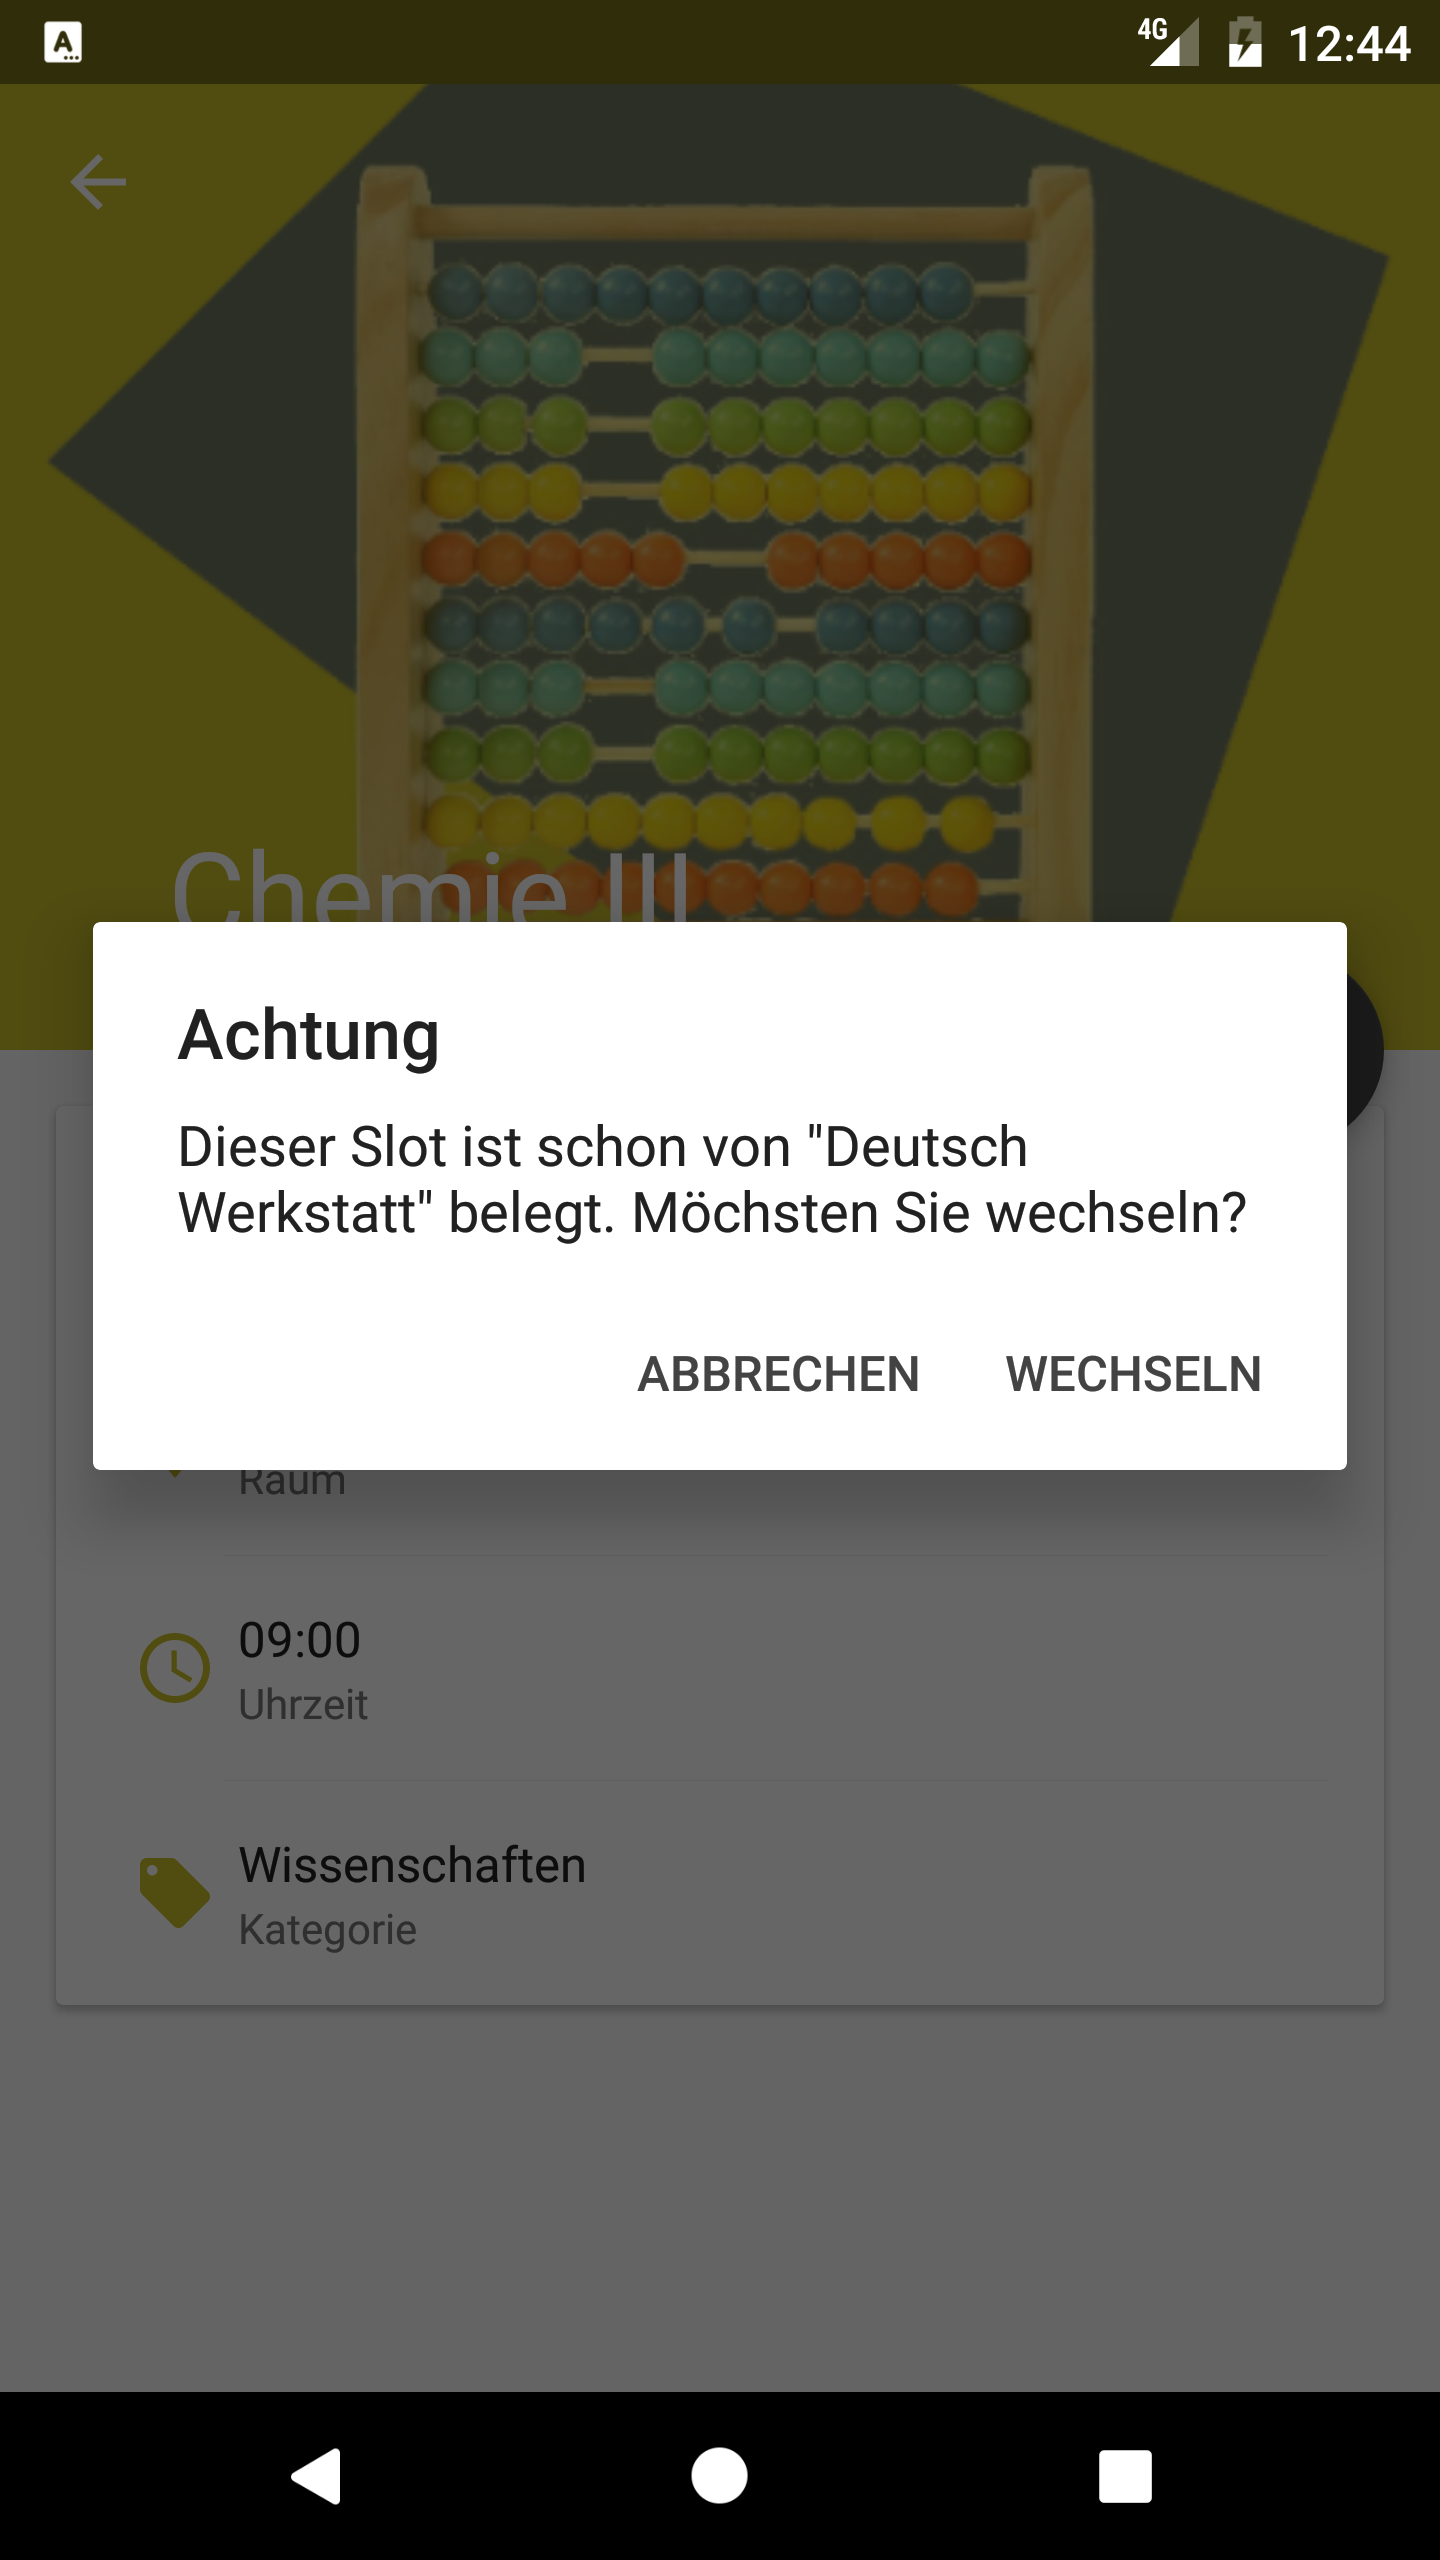
\includegraphics[scale=0.075]{screen_alert}
	\end{center}
	\caption{Warnhinweis}
	\label{fig:alert}
\end{figure}


\section{Timer}
\subsection{Service}
Diese Aufgabe wurde nicht durch einen Android-\inlinecode{Service} gelöst, sondern mit Hilfe der \inlinecode{AlarmManager}-API, mit der Ereignise in der Zukunft geplant werden können. Dies ist effektiver als für jede Markierung einen Service zu erstellen. Siehe \ref{ss:notification}. Das Öffnen des Angebots wurde durch eine Notifcation ersetzt.

\subsection{Aktion}
Siehe \ref{ss:notification}.


\section{Notification}
\subsection{Notification\label{ss:notification}}
Mit der statischen \inlinecode{scheduleNotification()}-Methode der Klasse \inlinecode{NotificationPublisher} werden Notifications für die entsprechenden Kurse zur jeweiligen Uhrzeit angelegt (Achtung: In Debug-Builds werden die Notifications, zur besseren Testbarkeit, abhängig von der aktuellen Uhrzeit angelegt). Da \inlinecode{NotificationPublisher} die abstrakte Klasse \inlinecode{BroadcastReceiver} erweitert, können auf die Alarme in \inlinecode{onReceive()} reagiert und die Notification gepublisht werden.

\subsection{Alarm}
\begin{sloppypar}
Das Abspielen des Wecktons wurde durch einen Android-\inlinecode{Service} gelöst, siehe \inlinecode{NotificationSoundService}, damit der Weckton bis zum Anklicken der Notification gespielt werden kann.
\end{sloppypar}

\end{document}
